\chapter{聚合物}\label{ch:g12:polymers}

抓绒外套可以用熔化的饮料瓶纺成；攀岩绳
由尼龙制成；这页纸是纤维素，由树木制成。三者都是
\omterm{def:g12:polymers:polymer}{聚合物}，即长达数千个\omterm{def:g7:atoms-and-molecules:atom}{原子}的\omterm{def:g7:atoms-and-molecules:molecule}{分子}，由一种小单元
不断重复连接而成。它们的性质——柔软还是坚硬、有弹性还是易碎、能否熔化——
与其说取决于所含的\omterm{def:g7:atoms-and-molecules:atom}{原子}，不如说更多取决于
长链的排列方式。

\begin{recall}
\omterm{def:g8:plastics:plastic}{塑料}由很长的\omterm{def:g7:atoms-and-molecules:molecule}{分子}组成；\omterm{def:g8:plastics:thermoplastic}{热塑性塑料}受热会软化，
\omterm{def:g8:plastics:thermoplastic}{热固性塑料}则不会（见\cref{ch:g8:plastics}）。醇、酸、酯、
胺和\omterm{def:g11:functional-groups:amine}{酰胺}\omterm{def:g11:functional-groups:functional-group}{官能团}（见\cref{ch:g11:functional-groups}）。加成反应是指
将两个\omterm{def:g7:atoms-and-molecules:molecule}{分子}结合为一个，且不失去任何\omterm{def:g7:atoms-and-molecules:atom}{原子}
（见\cref{ch:g12:curly-arrows}）。
\end{recall}

\begin{omfigure}
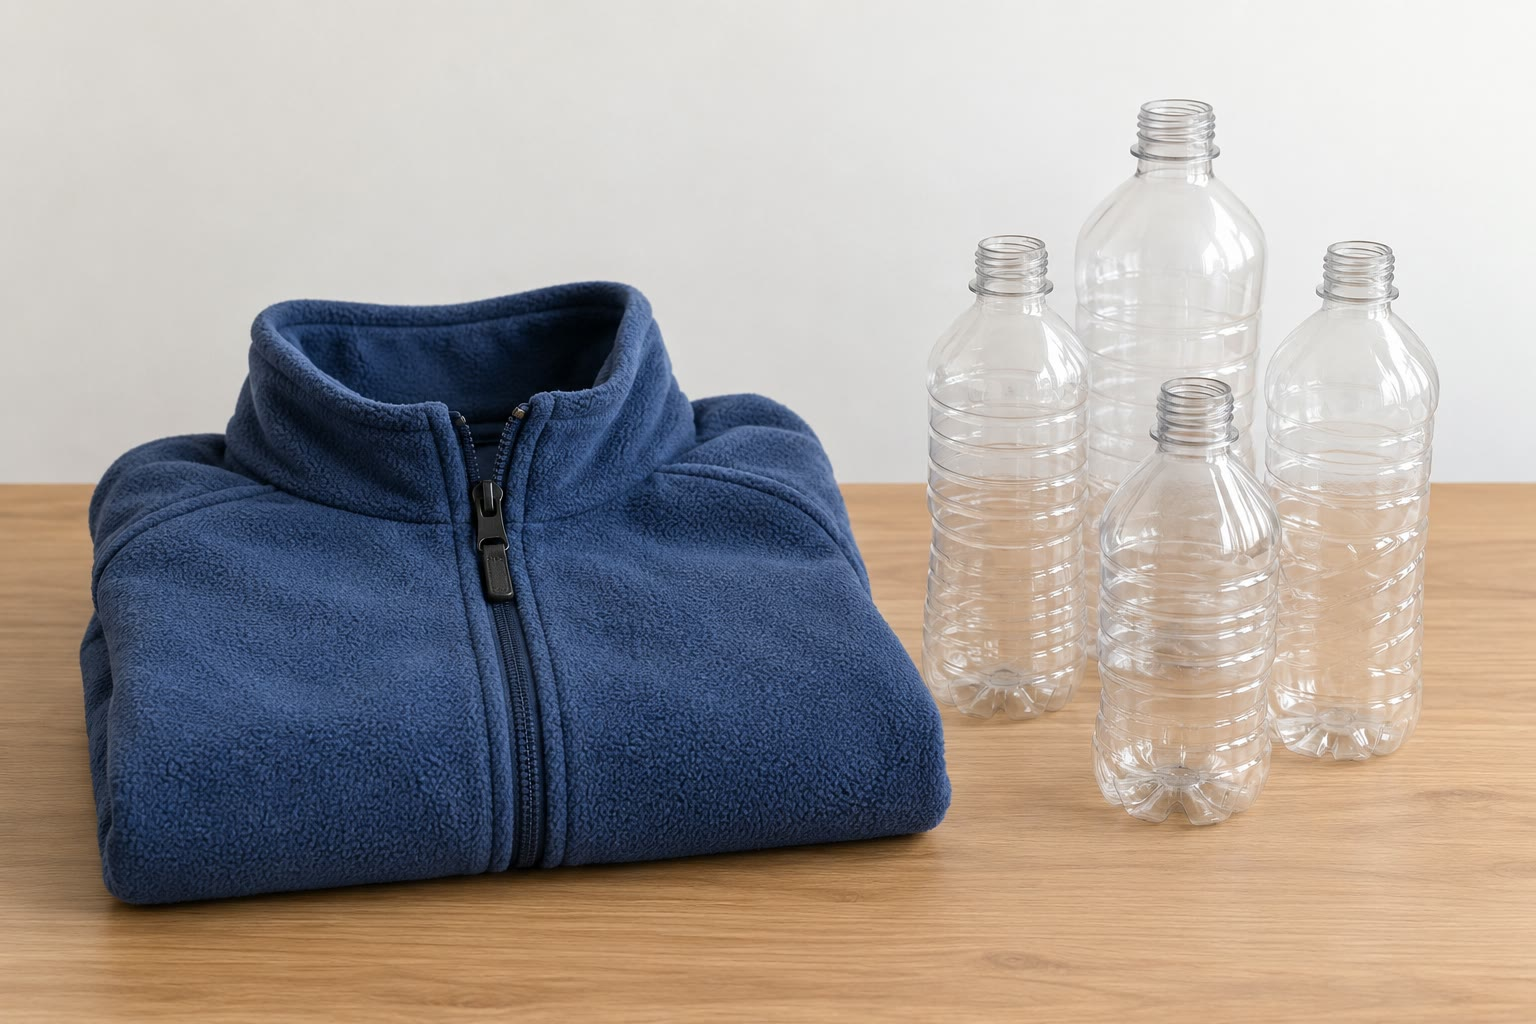
\includegraphics[width=0.45\linewidth]{images/book1/ai/g12-fleece-bottles.jpg}

{\small 用过的饮料瓶与抓绒外套：同一种\omterm{def:g12:polymers:polymer}{聚合物}的
两种形态。}
\end{omfigure}

\section{单体、聚合物、重复单元}

\begin{definition}[聚合物、单体、聚合反应]\label{def:g12:polymers:polymer}
称\emph{聚合物}\index{聚合物}为由很大的\omterm{def:g7:atoms-and-molecules:molecule}{分子}组成的物质，
这些大\omterm{def:g7:atoms-and-molecules:molecule}{分子}每个都由许多小单元依次连接而成。
组成它的小\omterm{def:g7:atoms-and-molecules:molecule}{分子}称为它的
\emph{单体}\index{单体}；将它们连接起来的反应称为
\emph{聚合反应}\index{聚合反应}。
\end{definition}

\begin{definition}[重复单元、聚合度]\label{def:g12:polymers:repeat-unit}
\omterm{def:g12:polymers:polymer}{聚合物}的\emph{重复单元}\index{重复单元}是
能通过重复得到整条链的最小\omterm{def:g7:atoms-and-molecules:atom}{原子}团，写在方括号内，
并标注\omterm{def:g7:atoms-and-molecules:formula}{下标} $n$。链中重复单元的数目 $n$ 称为
其\emph{聚合度}\index{聚合度}。
\end{definition}

\begin{omfigure}
\[
  n\;\ce{CH2=CH2}
  \quad\longrightarrow\quad
  \chemfig{-[@{op1,.75}]CH_2-CH_2-[@{cl1,0.25}]}
  \polymerdelim[height=6pt, depth=6pt, indice=n]{op1}{cl1}
\]

{\small 乙烯的\omterm{def:g12:polymers:polymer}{聚合反应}：$n$ 个\omterm{def:g12:polymers:polymer}{单体}\omterm{def:g7:atoms-and-molecules:molecule}{分子}生成一条
聚乙烯链，其\omterm{def:g12:polymers:repeat-unit}{重复单元} \ce{-CH2-CH2-} 写在
方括号内。}
\end{omfigure}

\begin{proposition}[聚合物的摩尔质量]\label{prop:g12:polymers:molar-mass}
\omterm{def:g12:polymers:repeat-unit}{聚合度}为 $n$ 的链，其\omterm{def:g10:the-mole:molar-mass}{摩尔质量}
\[
  M(\text{聚合物}) \approx n \times M(\text{重复单元}) ,
\]
链的两端在 $n$ 很大时可忽略不计。
\end{proposition}

\begin{proof}
链由 $n$ 个\omterm{def:g12:polymers:repeat-unit}{重复单元}和两个端基组成，每个端基只含几个\omterm{def:g7:atoms-and-molecules:atom}{原子}；
当 $n$ 为数千时，端基的质量不到
整个\omterm{def:g7:atoms-and-molecules:molecule}{分子}的千分之一。
\end{proof}

\begin{example}[一条聚乙烯链]\label{ex:g12:polymers:pe}
% ledger: aw:C, aw:H
一条\omterm{def:g10:the-mole:molar-mass}{摩尔质量}为 \qty{280000}{g/mol} 的聚乙烯链，
含 $n = 280000/28.0 = 10000$ 个\omterm{def:g12:polymers:repeat-unit}{重复单元}，因此连续排列着两万个碳\omterm{def:g7:atoms-and-molecules:atom}{原子}。
实际样品中，各条链的长度并不相同：
$n$ 是一个平均值。
\end{example}

\section{加聚物}

\begin{definition}[加聚物、缩聚物]\label{def:g12:polymers:addition-polymer}
称\emph{加聚物}\index{加聚物}是由\omterm{def:g12:polymers:polymer}{单体}通过加成反应形成的，
这些\omterm{def:g12:polymers:polymer}{单体}带有 \ce{C=C} \omterm{def:g10:lewis-and-shape:multiple-bond}{双键}，且不生成其他产物：其
\omterm{def:g12:polymers:repeat-unit}{重复单元}与\omterm{def:g12:polymers:polymer}{单体}的\omterm{def:g7:atoms-and-molecules:atom}{原子}组成相同。称\emph{缩聚
物}\index{缩聚物}是通过两个\omterm{def:g11:functional-groups:functional-group}{官能团}之间的反应形成的，
此类反应使两个\omterm{def:g12:polymers:polymer}{单体}连接，并在每个连接处放出一个小\omterm{def:g7:atoms-and-molecules:molecule}{分子}，
通常是水。
\end{definition}

\begin{omfigure}
\footnotesize
\renewcommand{\arraystretch}{1.5}
\begin{tabular}{l l l l}
\hline
\omterm{def:g12:polymers:polymer}{单体} & \omterm{def:g12:polymers:polymer}{聚合物} & \omterm{def:g12:polymers:repeat-unit}{重复单元} & 用途 \\
\hline
乙烯 \ce{CH2=CH2} & 聚乙烯 (PE) & \ce{-CH2-CH2-} & 袋子、瓶子 \\
氯乙烯 \ce{CH2=CHCl} & 聚氯乙烯 (PVC) & \ce{-CH2-CHCl-} & 管道、窗框 \\
苯乙烯 \ce{CH2=CH-C6H5} & 聚苯乙烯 (PS) & \ce{-CH2-CH(C6H5)-} & 杯子、泡沫 \\
四氟乙烯 \ce{CF2=CF2} & PTFE & \ce{-CF2-CF2-} & 不粘锅 \\
\hline
\end{tabular}\par\medskip

{\small 四种\omterm{def:g12:polymers:addition-polymer}{加聚物}。在每一种中，\omterm{def:g12:polymers:polymer}{单体}的\omterm{def:g10:lewis-and-shape:multiple-bond}{双键}
打开，其两个碳\omterm{def:g7:atoms-and-molecules:atom}{原子}并入链中。}
\end{omfigure}

\begin{method}[由聚合物求单体]\label{met:g12:polymers:monomer}
\begin{enumerate}
  \item 找出\omterm{def:g12:polymers:repeat-unit}{重复单元}：能通过重复得到
        整条链的最小\omterm{def:g7:atoms-and-molecules:atom}{原子}团。
  \item 若主链只含碳\omterm{def:g7:atoms-and-molecules:atom}{原子}，则为\omterm{def:g12:polymers:addition-polymer}{加聚物}，
        需在\omterm{def:g12:polymers:repeat-unit}{重复单元}主链的两个碳\omterm{def:g7:atoms-and-molecules:atom}{原子}间补回一个\omterm{def:g10:lewis-and-shape:multiple-bond}{双键}，
        这就是\omterm{def:g12:polymers:polymer}{单体}。
  \item 若主链含有酯基或\omterm{def:g11:functional-groups:amine}{酰胺}基连接，则为
        \omterm{def:g12:polymers:addition-polymer}{缩聚物}：断开每个连接，并将每一侧
        都归还所释放小\omterm{def:g7:atoms-and-molecules:molecule}{分子}的\omterm{def:g7:atoms-and-molecules:atom}{原子}（\ce{-OH} 接到
        \ce{C=O}，\ce{-H} 接到 \ce{O} 或 \ce{N}）。这些即为
        \omterm{def:g12:polymers:polymer}{单体}。
\end{enumerate}
\end{method}

\begin{example}[PVC 的单体]\label{ex:g12:polymers:pvc}
该链 \ce{-CH2-CHCl-CH2-CHCl-CH2-CHCl-} 由 \ce{-CH2-CHCl-} 重复构成；它
主链中只含碳\omterm{def:g7:atoms-and-molecules:atom}{原子}，故其\omterm{def:g12:polymers:polymer}{单体}为
\ce{CH2=CHCl}，即氯乙烯。
\end{example}

\section{缩聚物}

只含一个反应基团的\omterm{def:g12:polymers:polymer}{单体}只能成键一次：它会使链终止。
要通过缩聚形成长链，每个\omterm{def:g12:polymers:polymer}{单体}需要两个基团，
分别位于两端。

\begin{example}[PET，一种聚酯]\label{ex:g12:polymers:pet}
% ledger: aw:C, aw:H, aw:O
1,2-乙二醇 \ce{HO-CH2-CH2-OH}，含两个醇羟基；
对苯二甲酸 \ce{HOOC-C6H4-COOH}，含两个羧基。每个
羧基与一个醇羟基生成酯，同时释放出水：
链从两端同时增长。该\omterm{def:g12:polymers:polymer}{聚合物}为聚对苯二甲酸乙二醇酯，
PET，是饮料瓶和聚酯纤维的材料。其\omterm{def:g12:polymers:repeat-unit}{重复
单元} \ce{C10H8O4} 的\omterm{def:g10:the-mole:molar-mass}{摩尔质量}为 \qty{192.0}{g/mol}，即
两个\omterm{def:g12:polymers:polymer}{单体}的\omterm{def:g10:the-mole:molar-mass}{摩尔质量}之和（$62.0 + 166.0$）减去两\omterm{def:g7:atoms-and-molecules:molecule}{分子}水（$36.0$）。
\end{example}

\begin{omfigure}
\setchemfig{atom sep=1.9em}
\chemfig{HO-CH_2-CH_2-OH}
\quad $+$ \quad
\chemfig{HO-C(=[2]O)-*6(-=-(-C(=[2]O)-OH)=-=)}

\medskip
$\longrightarrow$\quad
\chemfig{-[@{op2,.75}]O-CH_2-CH_2-O-C(=[2]O)-*6(-=-(-C(=[2]O)-[@{cl2,0.25}])=-=)}
\polymerdelim[height=20pt, depth=6pt, indice=n]{op2}{cl2}
\quad $+\ 2n\ \ce{H2O}$

{\small 由两种\omterm{def:g12:polymers:polymer}{单体}生成 PET：每个酯键（\ce{-CO-O-}
基团）释放一\omterm{def:g7:atoms-and-molecules:molecule}{分子}水。}
\end{omfigure}

\begin{example}[尼龙-6,6，一种聚酰胺]\label{ex:g12:polymers:nylon}
己二胺（1,6-己二胺）\ce{H2N-(CH2)6-NH2} 与己二酸
\ce{HOOC-(CH2)4-COOH}，通过\omterm{def:g11:functional-groups:amine}{酰胺}键相连，每一步都释放一\omterm{def:g7:atoms-and-molecules:molecule}{分子}
水：
\[
  \cdots\ce{-NH-(CH2)6-NH-CO-(CH2)4-CO-}\cdots
\]
名称中的两个 6 表示每种\omterm{def:g12:polymers:polymer}{单体}中的碳\omterm{def:g7:atoms-and-molecules:atom}{原子}数。
相邻链的\omterm{def:g11:functional-groups:amine}{酰胺}键之间通过\omterm{def:g11:polarity-and-cohesion:hydrogen-bond}{氢键}相互吸引，
这使尼龙纤维强度很高。
\end{example}

\begin{history}[卡罗瑟斯与尼龙]
% ledger: hist:polyamides-1934, hist:nylon-production-1939
化学家华莱士·卡罗瑟斯，曾领导一家化工公司的
研究实验室，他着手证明\omterm{def:g12:polymers:polymer}{聚合物}确是巨大的
真实\omterm{def:g7:atoms-and-molecules:molecule}{分子}，并有意制造出它们。他的团队最先制得聚酯，
它们过易熔化而无实用价值；1934 年，他们转而使用胺，
制得聚\omterm{def:g11:functional-groups:amine}{酰胺}，其中一种后来被命名为尼龙的纤维。尼龙
于 1939 年投入生产，最初是在一次世界博览会上引起轰动的丝袜，
随后用于降落伞、绳索和牙刷刷毛。
\end{history}

\begin{omfigure}
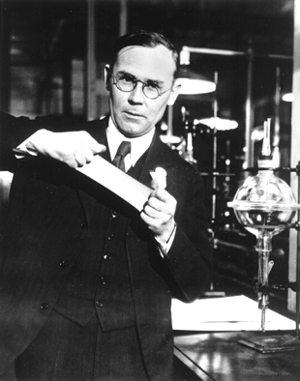
\includegraphics[width=0.24\linewidth]{images/book1/carothers.jpg}

{\small 华莱士·卡罗瑟斯在其实验室中。}
\end{omfigure}

\section{结构与性质}

同一种\omterm{def:g12:polymers:polymer}{聚合物}的两个样品，性能可能大不相同；
起决定作用的是链的长度、链的形状以及链的堆积方式。

\begin{proposition}[链与性质]\label{prop:g12:polymers:properties}
\begin{itemize}
  \item 链越长，缠结越多：材料越坚固，
        熔化温度更高。
  \item 线性的链可以在有序的
        \emph{结晶}区域中并排排列；支链则不能，
        仍保持无序，即\emph{非晶}。结晶区域使
        \omterm{def:g12:polymers:polymer}{聚合物}更致密、更坚硬，也更不透明。
  \item 仅靠\omterm{def:g7:atoms-and-molecules:molecule}{分子}间作用力并列在一起的链，加热时
        会相互滑过，该\omterm{def:g12:polymers:polymer}{聚合物}为\omterm{def:g8:plastics:thermoplastic}{热塑性塑料}。
        而以共价\emph{交联}相连的链则不能：该\omterm{def:g12:polymers:polymer}{聚合物}为
        \omterm{def:g8:plastics:thermoplastic}{热固性塑料}；若交联较少，则为类橡胶的弹性
        固体。
\end{itemize}
\end{proposition}

\begin{proof}
加热使链获得足够的能量，以克服它们之间的
\omterm{def:g7:atoms-and-molecules:molecule}{分子}间作用力（见\cref{ch:g11:polarity-and-cohesion}），
其强度弱于\omterm{def:g10:lewis-and-shape:covalent-bond}{共价键}；链与链之间接触越多，
所需能量越大。交联是共价的：断开它们会破坏
材料本身，而非使其熔化。
\end{proof}

\begin{omfigure}
\begin{tikzpicture}[font=\footnotesize, line width=1pt, line cap=round,
    lab/.style={below, align=center, text width=2.8cm}]
  % linear, packed (crystalline)
  \begin{scope}
    \foreach \y in {0,0.25,0.5,0.75,1.0}
      \draw[omDef] plot[smooth, domain=0:2.2, samples=25] (\x, {\y + 0.05*sin(400*\x)});
    \node[lab] at (1.1,-0.2) {线性链 \\ 整齐排列：结晶};
  \end{scope}
  % linear, tangled (amorphous)
  \begin{scope}[xshift=3.4cm]
    \draw[omDef] plot[smooth] coordinates {(0,0.2) (0.5,0.9) (1.0,0.3) (1.4,1.1) (2.0,0.5) (2.2,0.9)};
    \draw[omProp] plot[smooth] coordinates {(0,0.9) (0.4,0.3) (0.9,1.0) (1.5,0.2) (1.9,1.0) (2.2,0.3)};
    \draw[black!60] plot[smooth] coordinates {(0.1,0.55) (0.7,0.1) (1.2,0.75) (1.7,0.55) (2.2,0.1)};
    \node[lab] at (1.1,-0.2) {线性链 \\ 缠结：非晶};
  \end{scope}
  % branched
  \begin{scope}[xshift=6.8cm]
    \draw[omDef] plot[smooth] coordinates {(0,0.5) (0.6,0.6) (1.2,0.45) (1.8,0.65) (2.2,0.5)};
    \draw[omDef] (0.5,0.6) -- (0.35,1.05) (1.0,0.5) -- (1.15,0.05) (1.6,0.6) -- (1.5,1.1) (1.6,0.6) -- (1.95,1.0);
    \node[lab] at (1.1,-0.2) {支链：\\ 无法堆积};
  \end{scope}
  % cross-linked
  \begin{scope}[xshift=10.2cm]
    \foreach \y in {0.1,0.55,1.0}
      \draw[omDef] plot[smooth, domain=0:2.2, samples=25] (\x, {\y + 0.06*sin(300*\x)});
    \foreach \x/\a/\b in {0.4/0.1/0.55, 1.3/0.1/0.55, 0.9/0.55/1.0, 1.9/0.55/1.0}
      \draw[omProp, line width=1.6pt] (\x,\a) -- (\x,\b);
    \node[lab] at (1.1,-0.2) {交联链：\\ 不熔化};
  \end{scope}
\end{tikzpicture}

{\small 四种\omterm{def:g12:polymers:polymer}{聚合物}链的排列方式。交联（橙色）是
链与链之间的\omterm{def:g10:lewis-and-shape:covalent-bond}{共价键}。}
\end{omfigure}

\begin{example}[两种聚乙烯]\label{ex:g12:polymers:two-pe}
在极高压力下制得的聚乙烯带有许多短支链：
其\omterm{def:g7:atoms-and-molecules:molecule}{分子}链堆积不紧密，制成的薄膜柔软透明，常用于制袋。
用\omterm{def:g12:catalysis:catalyst}{催化剂}在低压下制得的聚乙烯，\omterm{def:g7:atoms-and-molecules:molecule}{分子}链几乎呈直线形，
并堆积成结晶区：密度更大、更硬，可制成牛奶瓶
和周转箱。二者\omterm{def:g12:polymers:polymer}{单体}相同、\omterm{def:g12:polymers:repeat-unit}{重复单元}相同，
只是结构不同。
\end{example}

\section{天然聚合物}

生物早在化学家之前就已\omterm{def:g10:synthesis-yield:synthesis}{合成}了\omterm{def:g12:polymers:polymer}{聚合物}。

\begin{itemize}
  \item \textbf{纤维素}和\textbf{淀粉}都是由葡萄糖
        单元连接成的链，每个单元为 \ce{C6H10O5}，连接方式不同：纤维素
        形成笔直而坚韧的纤维（木材、棉花、纸）；淀粉
        形成可被人体消化的卷曲链。
  \item \textbf{蛋白质}是由氨基酸通过\omterm{def:g11:functional-groups:amine}{酰胺}键连接成的链，
        即二肽的肽键（见
        \cref{ch:g12:synthesis-strategy}）。
  \item \textbf{DNA}是由核苷酸构成的链；其四种单元的
        排列顺序储存着遗传信息。
  \item \textbf{天然橡胶}是异戊二烯的\omterm{def:g12:polymers:addition-polymer}{加聚物}，
        \ce{CH2=C(CH3)-CH=CH2}，以乳白色液体（胶乳）形式
        从橡胶树的树皮中采集。与硫共热后，其\omterm{def:g7:atoms-and-molecules:molecule}{分子}链
        经硫桥交联，橡胶变得更坚韧，并能保持
        形状，如轮胎。
\end{itemize}

\begin{omfigure}
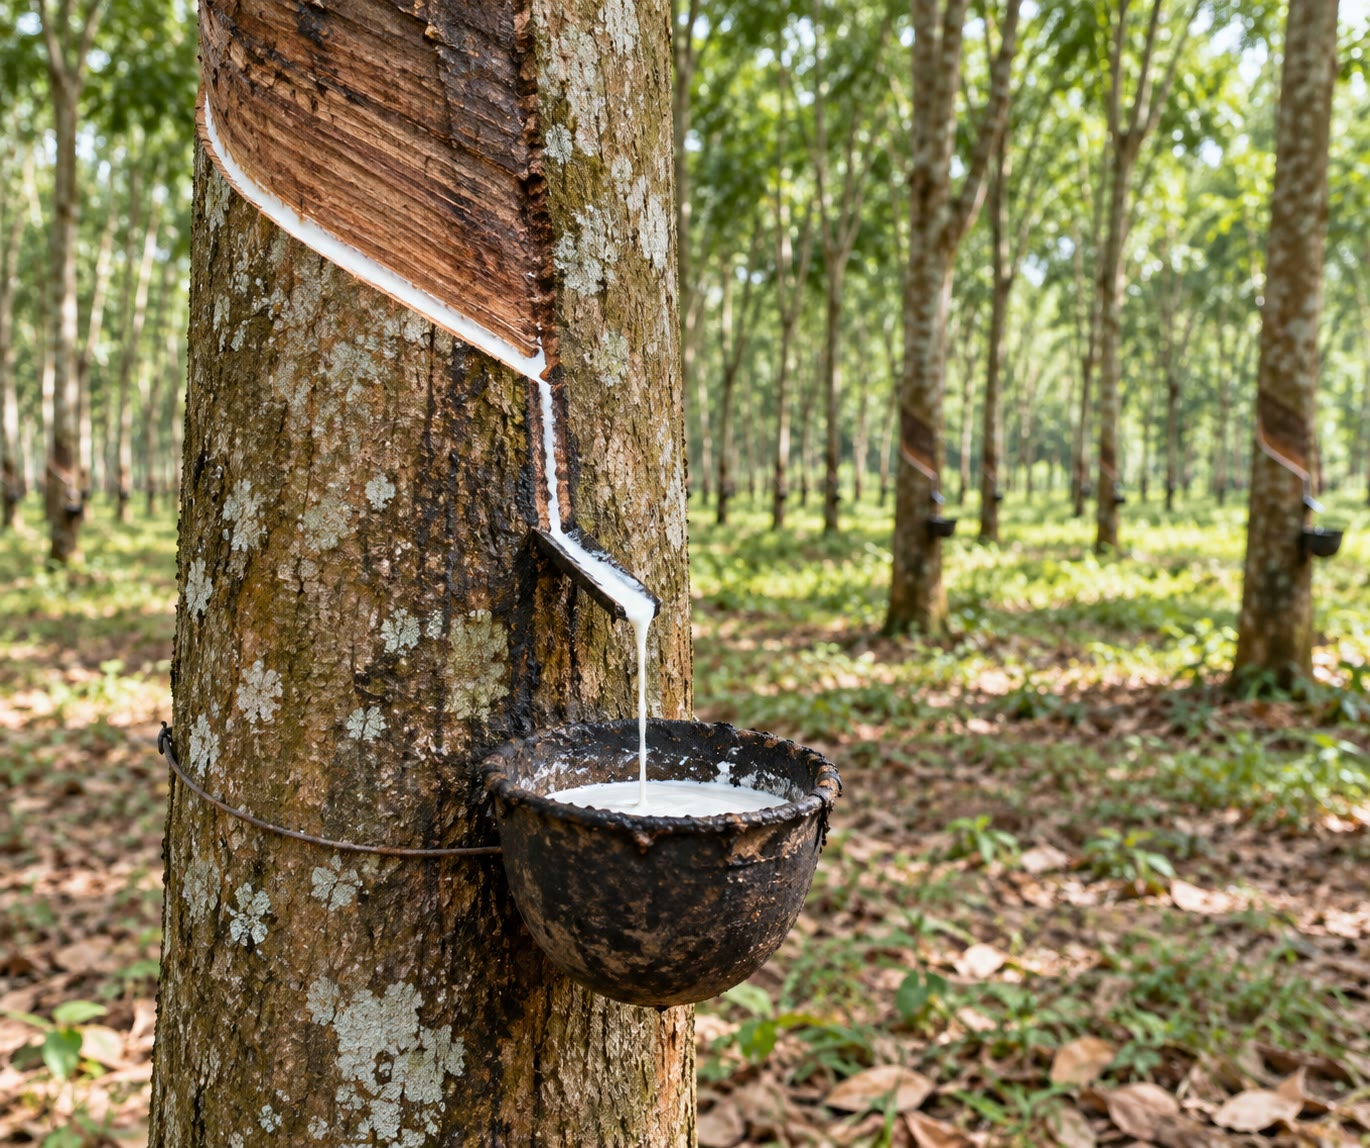
\includegraphics[width=0.45\linewidth]{images/book1/ai/g12-rubber-tapping.jpg}

{\small 割胶：胶乳从树皮切口流入
杯中。}
\end{omfigure}

\begin{remark}[制造与回收]\label{rem:g12:polymers:recycling}
\omterm{def:g8:plastics:thermoplastic}{热塑性塑料}可熔化后重新成型：机械回收。一种
\omterm{def:g12:polymers:addition-polymer}{缩聚物}还可借助
逆反应（即水解）分解为\omterm{def:g12:polymers:polymer}{单体}，再由\omterm{def:g12:polymers:polymer}{单体}制成新的\omterm{def:g12:polymers:polymer}{聚合物}：
化学回收。\omterm{def:g8:plastics:thermoplastic}{热固性塑料}两种回收都难以实现。
\end{remark}

\section{练习}

\begin{exercise}[$\star$]\label{exo:g12:polymers:1}
求聚丙烯的\omterm{def:g12:polymers:polymer}{单体}，其\omterm{def:g12:polymers:repeat-unit}{重复单元}为
\ce{-CH2-CH(CH3)-}。
\end{exercise}

\begin{exercise}[$\star$]\label{exo:g12:polymers:2}
写出由四氟乙烯（
\ce{CF2=CF2}）聚合而成的\omterm{def:g12:polymers:polymer}{聚合物}的\omterm{def:g12:polymers:repeat-unit}{重复单元}。它属于\omterm{def:g12:polymers:addition-polymer}{加聚物}还是\omterm{def:g12:polymers:addition-polymer}{缩聚物}？
\end{exercise}

\begin{exercise}[$\star$]\label{exo:g12:polymers:3}
判断下列\omterm{def:g12:polymers:polymer}{聚合物}是\omterm{def:g12:polymers:addition-polymer}{加聚物}还是\omterm{def:g12:polymers:addition-polymer}{缩聚物}：聚乙烯、PET、尼龙、
PVC、聚苯乙烯。
\end{exercise}

\begin{exercise}[$\star$]\label{exo:g12:polymers:4}
下列\omterm{def:g12:polymers:polymer}{聚合物}中哪些是天然的：纤维素、尼龙、淀粉、PVC、
胶乳制得的橡胶、蛋白质？
\end{exercise}

\begin{exercise}[$\star$]\label{exo:g12:polymers:5}
为什么\omterm{def:g12:polymers:addition-polymer}{缩聚物}的每个\omterm{def:g12:polymers:polymer}{单体}都必须带有两个
活性基团？
\end{exercise}

\begin{exercise}[$\star\star$]\label{exo:g12:polymers:6}
某 PVC 样品的平均\omterm{def:g10:the-mole:molar-mass}{摩尔质量}为 \qty{125000}{g/mol}。
求其\omterm{def:g12:polymers:repeat-unit}{聚合度}。
\end{exercise}

\begin{exercise}[$\star\star$]\label{exo:g12:polymers:7}
某聚苯乙烯链的\omterm{def:g12:polymers:repeat-unit}{聚合度}为 2500。计算
其\omterm{def:g10:the-mole:molar-mass}{摩尔质量}。
\end{exercise}

\begin{exercise}[$\star\star$]\label{exo:g12:polymers:8}
乳酸 \ce{CH3-CH(OH)-COOH} 含有一个醇羟基和
一个羧基。证明它能自身形成聚酯，写出其
\omterm{def:g12:polymers:repeat-unit}{重复单元}，并命名释放出的小\omterm{def:g7:atoms-and-molecules:molecule}{分子}。
\end{exercise}

\begin{exercise}[$\star\star$]\label{exo:g12:polymers:9}
结合链排列的图示，解释为什么制袋薄膜柔软
透明，而牛奶瓶却坚硬且不透明。
\end{exercise}

\begin{exercise}[$\star\star$]\label{exo:g12:polymers:10}
平底锅的把手是\omterm{def:g8:plastics:thermoplastic}{热固性塑料}，其\omterm{def:g8:plastics:plastic}{塑料}锅盖旋钮也是。描述
它们的\omterm{def:g7:atoms-and-molecules:molecule}{分子}链。为什么它们不能熔化后\omterm{def:g5:raw-materials-and-recycling:recycling}{回收利用}？
\end{exercise}

\begin{exercise}[$\star\star$]\label{exo:g12:polymers:11}
某尼龙-6,6 链的\omterm{def:g10:the-mole:molar-mass}{摩尔质量}为 \qty{22600}{g/mol}。计算
其\omterm{def:g12:polymers:repeat-unit}{重复单元} \ce{C12H22N2O2} 的\omterm{def:g10:the-mole:molar-mass}{摩尔质量}，再求其
\omterm{def:g12:polymers:repeat-unit}{聚合度}。
\end{exercise}

\begin{exercise}[$\star\star\star$]\label{exo:g12:polymers:12}
写出一\omterm{def:g7:atoms-and-molecules:molecule}{分子} 1,6-己二胺与一\omterm{def:g7:atoms-and-molecules:molecule}{分子}
己二酸之间的反应，生成第一个\omterm{def:g11:functional-groups:amine}{酰胺}键。为什么该产物
还能在两端继续反应？
\end{exercise}

\begin{exercise}[$\star\star\star$]\label{exo:g12:polymers:13}
制得 \qty{1.0}{kg} 尼龙-6,6 时，会释放出多少质量的水？
\end{exercise}

\begin{exercise}[$\star\star\star$]\label{exo:g12:polymers:14}
天然橡胶在温热时柔软发粘；与硫共热后，
变成轮胎所用的富有弹性、坚韧的橡胶。从\omterm{def:g7:atoms-and-molecules:molecule}{分子}链的角度加以解释。
为什么轮胎如此难以\omterm{def:g5:raw-materials-and-recycling:recycling}{回收利用}？
\end{exercise}

\begin{exercise}[$\star\star\star$]\label{exo:g12:polymers:15}
淀粉和纤维素的每个单元具有相同的化学式 \ce{C6H10O5}。
一条纤维素链的\omterm{def:g10:the-mole:molar-mass}{摩尔质量}为 \qty{1.6e6}{g/mol}，它含有多少个葡萄糖
单元？若每个单元使其长度增加 \qty{0.5}{nm}，
则该链有多长？
\end{exercise}

\section{问题：从瓶子到抓绒夹克}

\begin{problem}[{周末问题——一件抓绒夹克需要
多少个 25 g 的瓶子？}]
\label{pb:g12:polymers:1}
% ledger: aw:C, aw:H, aw:O
一件抓绒夹克由 \qty{300}{g} 的 PET 纤维制成。回收的废旧瓶子
每个 \qty{25}{g}，经收集、分拣、清洗、粉碎、熔融并纺丝；
在此过程中，瓶子质量的 \qty{80}{\percent} 最终成为
夹克中的纤维。

\medskip
\noindent\textbf{第一部分——\omterm{def:g12:polymers:polymer}{聚合物}。}
\begin{enumerate}
  \item 写出 PET 的两种\omterm{def:g12:polymers:polymer}{单体}，以及它们所带的
        \omterm{def:g11:functional-groups:functional-group}{官能团}。
  \item 二者之间形成何种键？释放出何种小\omterm{def:g7:atoms-and-molecules:molecule}{分子}？
  \item 判断 PET 是\omterm{def:g12:polymers:addition-polymer}{加聚物}还是\omterm{def:g12:polymers:addition-polymer}{缩聚物}？
  \item 计算两种\omterm{def:g12:polymers:polymer}{单体}的\omterm{def:g10:the-mole:molar-mass}{摩尔质量}。
  \item 推算\omterm{def:g12:polymers:repeat-unit}{重复单元} \ce{C10H8O4} 的\omterm{def:g10:the-mole:molar-mass}{摩尔质量}，
        并由其化学式加以核对。
\end{enumerate}

\medskip
\noindent\textbf{第二部分——链。}
\begin{enumerate}[resume]
  \item 一个瓶子中的 PET \omterm{def:g7:atoms-and-molecules:molecule}{分子}链，平均\omterm{def:g10:the-mole:molar-mass}{摩尔质量}为
        \qty{38400}{g/mol}。计算其\omterm{def:g12:polymers:repeat-unit}{聚合度}。
  \item 一条\omterm{def:g7:atoms-and-molecules:molecule}{分子}链大约含有多少个酯键？
  \item 瓶子的 PET 部分结晶。这说明
        其\omterm{def:g7:atoms-and-molecules:molecule}{分子}链有何特点？
  \item 为什么 PET 能够熔化并纺成纤维？
\end{enumerate}

\medskip
\noindent\textbf{第三部分——\omterm{def:g5:raw-materials-and-recycling:recycling}{回收利用}。}
\begin{enumerate}[resume]
  \item 制作一件夹克需要多少质量的瓶子？
  \item 这相当于多少个瓶子？
  \item 其余的质量去了哪里？
  \item 这种\omterm{def:g5:raw-materials-and-recycling:recycling}{回收利用}运用了\omterm{def:g12:synthesis-strategy:green-chemistry}{绿色化学}的哪一条原则？
\end{enumerate}

\medskip
\noindent\textbf{第四部分——回到\omterm{def:g12:polymers:polymer}{单体}。}
\begin{enumerate}[resume]
  \item 写出一个\omterm{def:g12:polymers:repeat-unit}{重复单元}水解生成
        各\omterm{def:g12:polymers:polymer}{单体}的\omterm{def:g8:balanced-equations:equation}{化学方程式}。
  \item \qty{1.00}{kg} PET 中含有多少\omterm{def:g10:the-mole:amount}{物质的量}的\omterm{def:g12:polymers:repeat-unit}{重复单元}？
  \item 将 \qty{1.00}{kg} PET 完全水解，
        可得各\omterm{def:g12:polymers:polymer}{单体}的质量分别为多少？
  \item 该过程消耗多少质量的水？请核对
        \omterm{def:g8:balanced-equations:conservation}{质量守恒}。
  \item 指出这种化学回收相对于熔融回收的一项优点。
  \item 给出最终答案：一件抓绒夹克
        需要多少个 \qty{25}{g} 的瓶子？
\end{enumerate}
\end{problem}
